%\documentclass[english, utf8]{article-hermes}
%\usepackage{listings}
%\usepackage[T1]{fontenc}
%\usepackage[frenchb]{babel}
%\usepackage{graphicx}
%\usepackage[labelfont=bf, labelsep=period]{caption}
%\usepackage{natbib}
%\usepackage{todonotes}
%\usepackage{amsmath}
%\usepackage{amssymb}
%\usepackage{algorithm}
%\usepackage[noend]{algpseudocode}
%\usepackage{hyperref}
%\usepackage[utf-8]{inputenc}



%\newcommand{\Section}[1]{section~\ref{#1}}
%\newcommand{\Sections}[2]{sections~\ref{#1}~and~\ref{#2}}
%\newcommand{\Figure}[1]{figure~\ref{#1}}
%\newcommand{\Table}[1]{Table~\ref{#1}}
%\newcommand{\Equation}[1]{Equation~(\ref{#1})}
%\newcommand{\ignore}[1]{}
%\providecommand{\keywords}[1]{\textbf{\textit{Keywords---}} #1}


%\journal{TAL.\ Volume 55--n$^{\circ}$3/2014}{73}{95}

\chapter{Learning word meanings from images of natural scenes}
\label{ch:TAL}
%\author{\'{A}kos K\'{a}d\'{a}r\fup{*} \andauthor Afra Alishahi\fup{*} \andauthor Grzegorz Chrupa\l{}a\fup{*}}
%\submitted[15/06/2015]{TAL~55-3}{R}

%\setcounter{page}{73}


\paragraph{Abstract}Children early on face
the challenge of learning the meaning of words
from noisy and ambiguous contexts.
Utterances that guide their learning are
emitted in complex scenes rendering the mapping between
visual and linguistic cues difficult. A key challenge in computational
modeling of the acquisition of word meanings is
to provide representations of scenes that
contain sources of information and statistical properties
similar in complexity to natural data. We propose a novel
computational model of cross-situational word learning
that takes images of natural scenes paired with
their descriptions as input and incrementally learns
probabilistic associations between words and image features.
Through a set of experiments we show
that the model learns meaning representations that correlate with human similarity
judgments, and that given
an image of a scene it produces words conceptually related to the image.

\newpage

\paragraph{This chapter is based on} Kadar, Á., Alishahi, A., \& Chrupala, G. (2015). 
Learning word meanings from images of natural scenes. \textit{Traitement Automatique des Langues.}

\newpage

%\keywords{Child language acquisition; Cross-situational learning; Computational cognitive modeling;
%Multi-modal learning.}
%\address{}
%\motscles{Acquisition du langage par l'enfant; apprentissage inter-situationnel;
%mod\'{e}lisation informatique et sciences cognitives; apprentissage multimodal}

%\resume{Les enfants sont très tôt confrontés au défi d'apprendre la signification des mots à partir de contextes bruités et ambigus. Les énoncés qui guident leur apprentissage sont émis au sein de scènes complexes qui rendent l'appariement entre indices visuels et linguistiques difficile. Un défi important de la modélisation informatique de l'acquisition du sens des mots réside en la proposition de représentations de scènes contenant des sources d'information et des propriétés statistiques %similaires en complexité à des données naturelles. Nous proposons un nouveau modèle d'apprentissage de mots inter-situationnel qui prend en entrée des images de scènes naturelles accompagnées de leurs descriptions et apprend incrémentalement des associations probabilistes entre mots et traits visuels. Nous montrons, à travers un ensemble d'expériences, que ce modèle apprend des représentations de sens corrélées aux jugements de similarité humains, et qu'il produit, pour une image de scène %donnée, des mots qui lui sont conceptuellement liés.}


%\address{%
%\fup{*} Tilburg Center for Cognition and Communication, Tilburg University}

%\date{31/03/2015 TAL~55-3}
%\begin{document}

%\maketitle



\section{Introduction}

Children learn most of their vocabulary from hearing words in noisy
and ambiguous contexts, where there are often many possible mappings
between words and concepts. They attend to the visual environment to
establish such mappings, but given that the visual context is often
very rich and dynamic, elaborate cognitive processes are required for
successful word learning from observation. Consider a language learner
hearing the utterance {\it ``the gull took my sandwich''} while
watching a bird stealing someone's food. For the word {\it gull}, such
information suggests potential mappings to the bird, the person, the
action, or any other part of the observed scene. Further exposure to
usages of this word and relying on structural cues from the sentence structure
is necessary to narrow down the range of its possible meanings.

%------------
\subsection{Cross-situational learning}
A well-established account of word learning from perceptual context is
called cross-situational learning, a bottom-up strategy in which the
learner draws on the patterns of co-occurrence between a word and its
referent across situations in order to reduce the number of possible
mappings \citep{Quine1960,Carey1978,pinker.89}. Various experimental
studies have shown that both children and adults use cross-situational
evidence for learning new words
\citep{yu.smith.07,smith.yu.08,vouloumanos.08,vouloumanos.werker.09}.

Cognitive word learning models have been extensively used to study how
children learn robust word-meaning associations despite the high rate
of noise and ambiguity in the input they receive. Most of the existing
models are either simple associative networks that gradually learn to
predict a word form based on a set of semantic features
\citep{Li.etal.2004,regier.05}, or are rule-based or
probabilistic implementations which use statistical regularities
observed in the input to detect associations between linguistic labels
and visual features or concepts
\citep{siskind.96,frank.etal.07,yu.08,fazly.etal.10csj}.
These models all implement different (implicit or explicit) variations
of the cross-situational learning mechanism, and demonstrate its
efficiency in learning robust mappings between words and meaning
representations in presence of noise and perceptual ambiguity.

However, a main obstacle to developing realistic models of child word
learning is lack of resources for reconstructing perceptual
context. The input to a usage-based cognitive model must contain the
same information components and statistical properties as
naturally-occurring data children are exposed to. A large collection
of transcriptions and video recordings of child-adult interactions has
been accumulated over the years \citep{macwhinney2014childes}, but few
of these resources provide adequate semantic annotations that can be
automatically used by a computational model. As a result, the existing
models of word learning have relied on artificially generated
input \citep{siskind.96}. The meaning of each word is represented as a symbol or a set of
semantic features that are selected arbitrarily or from lexical
resources such as WordNet \citep{fellbaum1998wordnet}, and the visual
context is built by sampling these symbols. Some models add additional noise
to data by randomly adding or removing meaning symbols to/from the perceptual
input \citep{fazly.etal.10csj}.

Carefully constructed artificial input is useful in testing the
plausibility of a learning mechanism, but comparisons with manually
annotated visual scenes show that these artificially generated data
sets often do not show the same level of complexity and ambiguity as
naturally occurring perceptual context
\citep{matusevych2013automatic,beekhuizen2013word}.

%------------
\subsection{Learning meanings from images}
\label{subsec:meanings-from-images}
To investigate the plausibility of cross-situational learning in a
more naturalistic setting, we propose to use visual features from
collections of images and their captions as input to a word learning
model.
%
In the domain of human-computer interaction (HCI) and robotics, a
number of models have investigated the acquisition of terminology for
visual concepts such as color and shape from visual data. Such
concepts are learned based on communication with human users
\citep{FleischmanRoy2005,skocaj2011system}.  Because of the HCI
setting, they need to make simplifying assumptions about the level of
ambiguity and uncertainty about the visual context.

The input data we exploit in this research has been used for much
recent work in NLP and machine learning whose goal is to develop
multimodal systems for practical tasks such as automatic image
captioning. This is a fast-growing field and a detailed discussion of
it is beyond the scope of this paper. Recent systems include
\cite{karpathy2014deep}, \cite{mao2014explain},
\cite{kiros2014unifying}, \cite{donahue2014long}, \cite{vinyals2014show},  \cite{venugopalan2014translating}, \cite{chen2014learning},  \cite{fang2014captions}. The majority of these
approaches rely on convolutional neural networks for deriving
representations of visual input, and then generate the captions using
various versions of recurrent neural network language models
conditioned on image representations. For example
\cite{vinyals2014show} use the deep convolutional neural network of
\cite{szegedy2014going} trained on ImageNet to encode the image into a
vector. This representation is then decoded into a sentence using a
Long Short-Term Memory recurrent neural network
\citep{hochreiter1997long}. Words are represented by embedding them
into a multidimensional space where similar words are close to each
other. The parameters of this embedding are trainable together with
the rest of the model, and are analogous to the vector representations
learned by the model proposed in this paper. The authors show some
example embeddings but do not analyze or evaluate them quantitatively,
as their main focus is on the captioning performance.

Perhaps the approach most similar to ours is the model of
\cite{bruni2014multimodal}. In their work, they train multimodal
distributional semantics models on both textual information and
bag-of-visual-words features extracted from captioned images. They use
the induced semantic vectors for simulating word similarity judgments
by humans, and show that a combination of text and image-based vectors
can replicate human judgments better than using uni-modal
vectors. This is a batch model and is not meant to simulate human word
learning from noisy context, but their evaluation scheme is suitable
for our purposes.

\cite{lazaridou2015combining} propose a multimodal model which learns
word representations from both word co-occurrences and from visual
features of images associated with words. Their input data consists of
a large corpus of text (without visual information) and additionally
of the ImageNet dataset \citep{deng2009imagenet} where images are
labeled with WordNet synsets.\label{rev:synset}\footnote{The synsets
of WordNet are groups of synonyms that represent an abstract concept.}
Thus, strictly speaking their model does
not implement cross-situational learning because a subset of words is
unambiguously associated with certain images.


%------------
\subsection{Our study}
\label{sec:out-study}

In this paper we investigate the plausibility of cross-situational
learning of word meanings in a more naturalistic setting. Our goal is
to simulate this mechanism under the same constraints that humans face
when learning a language, most importantly by learning in a piecemeal
and incremental fashion, and facing noise and ambiguity in their
perceptual environment. (We do not investigate the role of sentence structure on word learning in this study, but we discuss this issue in Section~\ref{sec:discussion}).
\label{why-incremental}

For simulation of the visual context we use two collections of images
of natural scenes, Flickr8K (F8k) \citep{rashtchian2010collecting} and
Flickr30K (F30k) \citep{young2014image}, where each image is associated with
several captions describing the scene. We extract visual features from
the images and learn to associate words with probability distributions
over these features. This has the advantage that we do not need to
simulate ambiguity or referential uncertainty -- the data has these
characteristics naturally.

The challenge is that, unlike in much previous work on
cross-situational learning of word meanings, we do not know the
ground-truth word meanings, and thus cannot directly measure the
progress and effectiveness of learning. Instead, we use indirect
measures such as (i) the correlation of the similarity of learned word
meanings to word similarities as judged by humans, and (ii) the
accuracy of producing words in response to an image. Our results show
that from pairings of scenes and descriptions it is feasible to learn
meaning representations that approximate human similarity
judgments. Furthermore, we show that our model is able to name image
descriptors considerably better than the frequency baseline and names
a large variety of these target concepts. In addition we present a
pilot experiment for word production using the ImageNet data set and
qualitatively show that our model names words that are conceptually
related to the images.



\section{Word learning model}
\label{sec:models}
Latest existing cross-situational models formulate word learning as a
translation problem, where the learner must decide which words in an
utterance correspond to which symbols (or potential referents) in the
perceptual context \cite{yu2007unified,fazly.etal.10csj}. For each new
utterance paired with a symbolic representation of the visual scene,
first the model decides which word is {\it aligned} with which symbol
based on previous associations between the two. Next, it uses the
estimated alignments to update the meaning representation associated
with each word.

We introduce a novel computational model for cross-situational word
learning from captioned images. We reformulate the problem of learning
the meaning of words as a translation problem between words and a {\it
  continuous} representation of the scene; that is, the visual
features extracted from the image. In this setting, the model learns
word representations by taking images and their descriptions one pair
at a time. To learn correspondences between English words and image
features, we borrow and adapt the translation-table estimation
component of the IBM Model 1 \cite{BrownPPM94}. The learning results
in a translation table between words and image-features, i.e.\ a list
of probabilities of image-features given a word.

\subsection{Visual input}
The features of the images are extracted by training a 16-layer
convolutional neural network (CNN) \cite{simonyan2014very} on an
object recognition task.\label{rev:cnndetail}\footnote{We used the F8k
  and F30k features available at
  \url{http://cs.stanford.edu/people/karpathy/deepimagesent/} and the
  data handling utilities from
  \url{https://github.com/karpathy/neuraltalk} for our
  experiments. The pre-trained CNN can be used through the Caffe
  framework \cite{jia2014caffe} and is available at the ModelZoo
  \url{https://github.com/BVLC/caffe/wiki/Model-Zoo}.} The network is
trained to discriminate among 1,000 different object labels on the
ImageNet dataset \cite{deng2009imagenet}. The last layer of the CNN
before the classification layer contains high level visual features of
the images, invariant to particulars such as position, orientation or
size.  We use the activation vector from this layer as a
representation of the visual scene described in the corresponding
caption. Each caption is paired with such a 4,096-dimensional vector
and used as input to a cross-situational word learner.
Figure~\ref{fig:dims} shows three sample images from the F8k
dataset most closely aligned with a particular dimension, as measured
by the cosine similarity between the image and a unit vector parallel
to the dimension axis. For example, dimension 1,000 seems to be related
to water, 2,000 to dogs or perhaps grass, and 3,000 to children.

 \begin{figure}
   \centering
   \begin{tabular}{c|lll}
     {\bf Dimension} & \multicolumn{3}{l}{\bf Top 3 images} \\\hline & & & \\
     1,000
     & 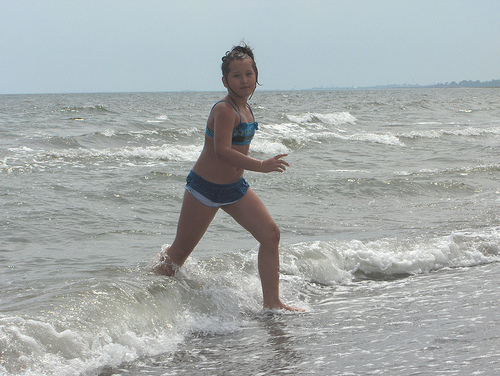
\includegraphics[height=1.5cm]{chapters/TAL/flickr8k/2726262796_03bd63a155.jpg}
     & 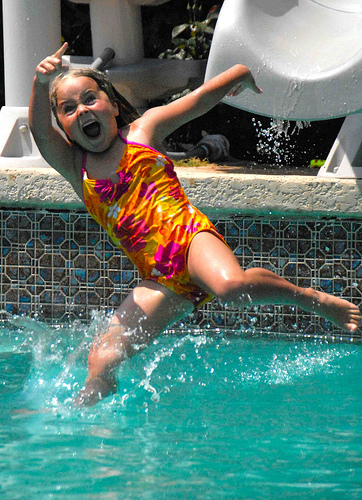
\includegraphics[height=1.5cm]{chapters/TAL/flickr8k/497122685_a51b29dc46.jpg}
     & 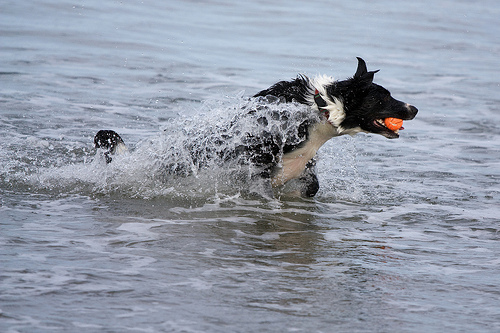
\includegraphics[height=1.5cm]{chapters/TAL/flickr8k/3515904775_f8acc5909e.jpg}
     \\
     & & & \\
     \hline
     & & & \\
     2,000
     & 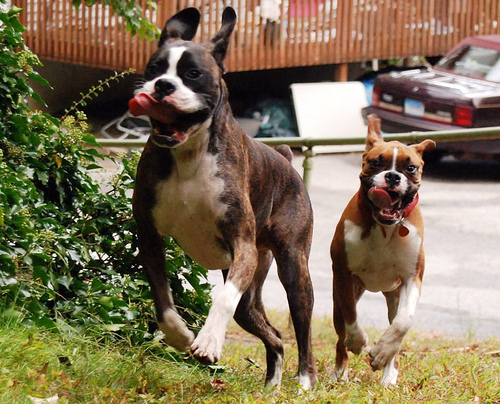
\includegraphics[height=1.5cm]{chapters/TAL/flickr8k/255741044_1102982213.jpg}
     & 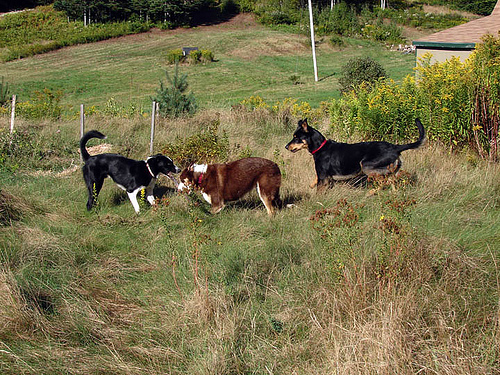
\includegraphics[height=1.5cm]{chapters/TAL/flickr8k/1388970365_162edcceb4.jpg}
     & 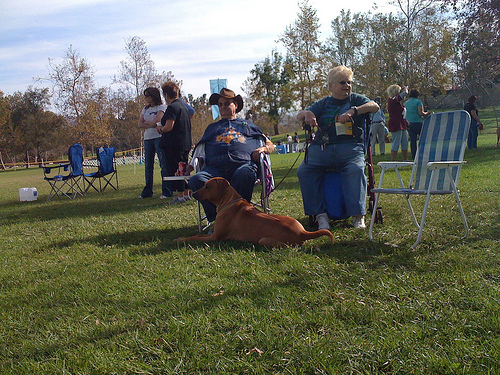
\includegraphics[height=1.5cm]{chapters/TAL/flickr8k/3053813297_7ce5f87710.jpg}
     \\
     & & & \\
     \hline
     & & & \\
     3,000
     & 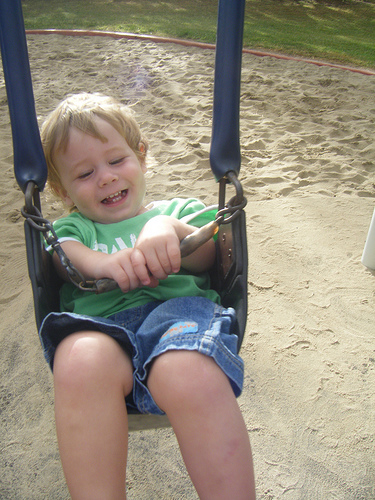
\includegraphics[height=1.5cm]{chapters/TAL/flickr8k/2362481035_a7600875d0.jpg}
     & 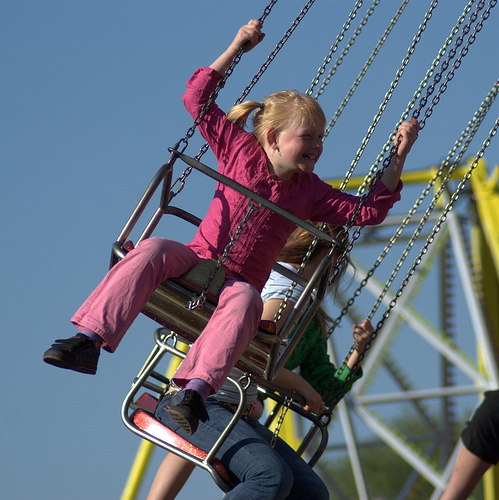
\includegraphics[height=1.5cm]{chapters/TAL/flickr8k/3504940491_94c43792ed.jpg}
     & 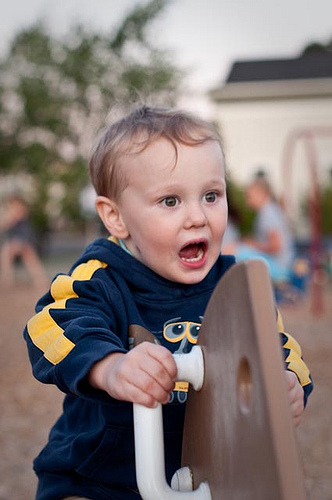
\includegraphics[height=1.5cm]{chapters/TAL/flickr8k/3751594676_edfbfa0688.jpg}
     \\
     & & & \\
     \hline
   \end{tabular}
   \caption{\textit{Dimensions with three most closely aligned images from F8k.}}
   \label{fig:dims}
 \end{figure}


 \subsection{Learning algorithm}
 We adapt the IBM model 1 estimation algorithm in the following
 ways\footnote{The source code for our model is available at
   \url{https://github.com/kadarakos/IBMVisual}.}: (i) like
 \citep{fazly.etal.10csj} we run it in an online fashion, and (ii)
 instead of two sequences of words, our input consists of one sequence
 of words on one side, and a vector of real values representing the
 image on the other side. The dimensions are indexes into the visual
 feature ``vocabulary'', while the values are interpreted as weights
 of these ``vocabulary items''. In order to get an intuitive
 understanding of how the model treats the values in the feature
 vector, we could informally liken these weights to word counts.  As
 an example consider the following input with a sentence and a vector
 of 5 dimensions (i.e.\ 5 features):
\begin{itemize}
\item The blue sky
\item $(2, 0, 2, 1, 0)$
\end{itemize}
Our model treats this equivalently to the following input, with the
values of the dimensions converted to ``feature occurrences'' of each
feature $f_n$.
\begin{itemize}
\item The blue sky
\item $f_1~f_1~f_3~f_3~f_4$
\end{itemize}

The actual values in the image vectors are always non-negative, since
they come from a rectified linear (ReLu) activation. However, they can
be fractional, and thus strictly speaking cannot be literal counts. We
simply treat them as generalized, fractional feature ``counts''.  The
end result is that given the lists of words in the image descriptions
and the corresponding image vectors the model learns a probability
distribution $t(f|w)$ over feature-vector indexes $f$ for every word
$w$ in the descriptions.


\begin{algorithm}
\caption{Sentence-vector alignment model
  (\textsc{Visual})}
\label{algo:ibm-vec}
\begin{algorithmic}[1]
\State { {\bf Input:} visual feature vectors paired with sentences
  $((V_1,S_1),\ldots,(V_N,S_N))$ }
\State { {\bf Output:} translation table $t(f|w)$ }
\State { $D \leftarrow $ dimensionality of feature vectors }
\State { $\epsilon \leftarrow 1$ } \Comment {Smoothing coefficient}
\State { $a[f,w] \leftarrow 0,~ \forall f,w$ } \Comment {Initialize count tables }
\State { $a[\cdot,w] \leftarrow 0,~ \forall w$ }
\State { $t(f|w) \leftarrow \frac{1}{D}$ }
\Comment{ Translation probability $t(f|w)$ }
\For {each input pair (vector $V$, sentence $S$)}
   \For {each feature index $f \in \{1,\ldots,D\}$}
        \State { $Z_f \gets \sum_{w \in S} t(f|w)$ } \Comment { Normalization constant $Z_f$ }
        \For { each word $w$ in sentence $S$}
           \State { $c \gets \frac{1}{Z_f} \times V[f] \times
             t(f|w)$ } \Comment { Expected count $c$ }
           \State { $a[f,w] \gets a[f,w] + c$ }
           \State { $a[\cdot,w] \gets a[\cdot,w] + c$ }
           \Comment { Updates to count tables }
           \State { $t(f|w) \leftarrow \frac{a[f,w]+\epsilon}{a[\cdot,w]+\epsilon D}$ }
           \Comment { Recompute translation probabilities }
\EndFor
\EndFor
\EndFor

\end{algorithmic}
\end{algorithm}

This is our sentence-vector alignment model, \textsc{Visual}. In the
interest of cognitive plausibility, we train it using a single-pass,
online algorithm. Algorithm~\ref{algo:ibm-vec} shows the pseudo-code.
Our input is a sequence of pairs of $D$-dimensional feature vectors
and sentences, and the output is a translation table $t(f|w)$. We
maintain two count tables of expected counts $a[f,w]$ and $a[\cdot,w]$
which are used to incrementally recompute the translation
probabilities $t(f|w)$. The initial translation probabilities are
uniform \mbox{(line 7)}. In lines 12-14 the count tables are updated, based
on translation probabilities weighted by the feature value $V[f]$, and
normalized over all the words in the sentence. In line 15 the
translation table is in turn updated.

\subsection{Baseline models}
\label{sec:baseline}

To asses the quality of the meaning representations learned by our
sentence-vector alignment model \textsc{Visual}, we compare its
performance in a set of tasks to the following baselines:
\begin{itemize}
  \item \textsc{Monoling:} instead of aligning each sentence with its
    corresponding visual vector, this variation aligns two copies of
    each sentence with each other, and thus learns word
    representations based on word-word co-occurrences\footnote{This
      model does not estimate probabilities of translation of a word
      to itself, that is probabilities of the form $t(w|w)$.}.
  \item \textsc{Word2Vec:} for comparison we also report results with the skip-gram embedding model, also known as \textsc{word2vec} which builds word
    representations based on word-word co-occurrences as well
    \cite{mikolov2013efficient,mikolov2013distributed}. \textsc{Word2vec}
    learns a vector representation (embedding) of a word which
    maximizes performance on predicting words in a small window around
    it.
\end{itemize}

\section{Experiments}
\label{sec:experiments}


\subsection{Image datasets}
\label{sec:dataset}
We use image-caption datasets for our experiments.
F8k \citep{rashtchian2010collecting} consists of 8000 images and five
captions for each image. F30k \citep{young2014image} extends the F8k and contains 31,783 images
with five captions each summing up to 158,915 sentences. For both data
sets we use the splits from \cite{karpathy2014deep}, leaving out 1000
images for validation and 1000 for testing from each
set. Table~\ref{tab:flickr} summarizes the statistics of the Flickr
image-caption datasets.



\begin{table}[h]
\centering
\begin{tabular}{l|r|r}
                    & F8k    & F30k   \\ \hline
Train images        & 6,000       & 29,780  \\
Validation images   & 1,000       & 1,000   \\
Test images         & 1,000       & 1,000   \\
Image in total      & 8,000       & 31,780  \\
Captions per image  & 5           & 5      \\
Captions in total   & 40,000      & 158,900 \\
\end{tabular}
\caption{\textit{Flickr image caption datasets.}}
\label{tab:flickr}
\end{table}
For the Single-concept image descriptions experiments reported in
section \ref{sec:experiments-production}, we also use the ILSVRC2012
subset of ImageNet \citep{russakovsky2015imagenet}, a widely-used data set in the computer vision
community. It is an image database that annotates the WordNet noun
synset hierarchy with images. It contains 500 images per synset on
average.

\subsection{Word similarity experiments}
\label{sec:experiments-wsj}
A common evaluation task for assessing the quality of learned semantic
vectors for words is measuring word similarity. A number of
experiments have elicited human ratings on the similarity and/or
relatedness of a list of word pairs. For instance one of the data sets
we used was the SimLex999 data set, which contains similarity judgments
for 666 noun pairs (organ-liver 6.15), 222 verb pairs (occur-happen 1.38)
and \mbox{111 adjective pairs} (nice-cruel 0.67) elicited by 500 participants
recruited from \mbox{Mechanical Turk}\label{rev:similarity_example}.
These types of data sets are commonly used as
benchmarks for models of distributional semantics, where the learned
representations are expected to show a significant positive
correlation with human similarity judgments on a large number of word
pairs.


We selected a subset of the existing benchmarks according to the size
of their word pairs that overlap with our restricted vocabulary. We
ran a statistical power analysis test to estimate the minimum number
of required word pairs needed in our experiments. The projected sample
size was $N=210$ with $p=.05$, effect-size $r=.2$ and
$\mathit{power}=0.9$.  Thus some of the well-known benchmarks were
excluded due to their small sample size after we excluded words not
present in our datasets.\footnote{These include RG-65
  \citep{rubenstein1965contextual}, MC-30 \citep{miller1991contextual}
  and YP-130 \citep{yang2006verb}.}


The four standard benchmarks that contain the minimum number of word
pairs are: the full WS-353 \citep{finkelstein2001placing}, MTurk-771
\citep{radinsky2011word}, MEN \citep{bruni2014multimodal} and
SimLex999 \citep{hill2015simlex}. Note that the MTurk dataset only
contains similarity judgments for nouns. Also, a portion of the full
WordSim-353 dataset reports relatedness ratings instead of word
similarity.

\subsection{Effect of concreteness on similarity judgments}
\label{sec:effect-concrete}
The word similarity judgments provide a macro evaluation about the
overall quality of the learned word representations. For more
fine-grained analysis we turn to the dichotomy of concrete (e.g.\ {\it
  chair, car}) versus abstract (e.g.\ {\it love, sorrow}) nouns.
Evidence presented by \cite{recchia2012semantic} shows that in naming
and lexical decision tasks the early activation of abstract concepts
is facilitated by rich linguistic contexts, while physical contexts
promote the activation of concrete concepts. Based on these recent
findings, \cite{bruni2014multimodal} suggest that in case of
computational models {\it concrete} words (such as names for physical
objects and visual properties) are easier to learn from
perceptual/visual input and {\it abstract} words are mainly learned
based on their co-occurrence with other words in text.  Following
\cite{bruni2014multimodal}, but using novel methodology, we also test
this idea and examine whether more concrete words benefit more from
visual features compared with less concrete ones.

In their work \cite{bruni2014multimodal} use the automatic method from \cite{turney2011literal}
to assign concreteness values to words and split the MEN corpus in
concrete and abstract chunks. From their experiments they draw the
conclusion that visual information boosts their models' performance on
concrete nouns. However, whereas the multi-modal embeddings of
\cite{bruni2014multimodal} are trained using an unbalanced corpus of
large quantities of textual information and far poorer visual stimuli,
our visual embeddings are learned on a parallel corpus of sentences
paired with images. To our purposes, this balance in the sources of
information is critical as we aim at modeling word learning in humans.
As a consequence of this setting we rather hypothesized that solely relying on visual features would result
in better performance on more concrete words than on abstract ones and
conversely, learning language solely from textual features would lead to
higher correlations on the more abstract portion of the vocabulary.

To test this hypothesis, MEN, MTurk and Simlex999 datasets were
split in two halves based on concreteness score of the word pairs.
The "abstract" and "concrete" subclasses for each data set are obtained
by ordering the pairs according to their concreteness and then partition
the ordered tuples in halves\label{rev:partition_concreteness}.
We defined the concreteness of a word pair as the product of the
concreteness scores of the two words. The scores are taken from
the University of South Florida
Free Association Norms dataset \citep{nelsonuniversity}.
Table~\ref{tab:benchmarks} provides an overview of the benchmarks we use in this study.
Column "Concreteness" shows the average concreteness scores of all words pairs per data set,
while columns "Concrete" and "Abstract" contain the average concreteness of the concrete
and abstract halves of the word-pairs respectively.


\begin{table}[h]
\tabcolsep=0.11cm
\centering
\begin{tabular}{@{}lrrr||rrr@{}}
\hline
 & \multicolumn{3}{c}{\#Pairs} &  \multicolumn{3}{c}{Concreteness} \\
\hline
\hline
               & Total & F8k & F30k  & Full set & Concrete & Abstract \\ \hline
 WS353   & 353   & 104              & 232               & 25.09        & 35.44 & 16.22 \\
 SimLex999   & 999   & 412              & 733               & 23.86        & 35.72 & 11.99 \\
 MEN          & 3000  & 2069             & 2839              & 29.77        & 36.28 & 23.26 \\
 MTurk771    & 771   & 295              & 594               & 25.89        & 34.02 & 16.16 \\
\hline
\end{tabular}
\caption{\textit{Summary of the word-similarity benchmarks, showing the number of
word pairs in the benchmarks and the size of their overlap with the F8k
and F30k data sets. The table also reports the average concreteness of
the whole, concrete and abstract portions of the benchmarks.}}
\label{tab:benchmarks}
\end{table}
%As demonstrated in \Figure{fig:concreteness}, our hypothesis was
%confirmed only in case of the MEN benchmark.

\subsection{Word production}
\label{sec:experiments-production}
Learning multi-modal word representations gives us the advantage of
replicating real-life tasks such as naming visual entities. In this
study, we simulate a word production task as follows: given an image
from the test set, we rank all words in our vocabulary according to
their cosine similarity to the visual vector representing the
image. We evaluate these ranked lists in two different ways.

\subsubsection{Multi-word image descriptions.}
We use images from the test portion of the F8k and F30k datasets as
benchmarks. These images are each labeled with up to five captions, or
multi-word descriptions of the content of the image. To evaluate the
performance of our model in producing words for each image, we
construct the target description of an image as the union of the words
in all its captions \label{rev:stopword}
(with stop-words\footnote{Function words such as \emph{the, is, at, what, there};
we used the stop-word list from the Python library NLTK.} removed). We compare this set
with the top $N$ words in our predicted ranked word list.
As a baseline for this experiment we implemented a simple frequency baseline
\textsc{Freq}, which for every image retrieves the top $N$ most frequent words.
The second model \textsc{Cosine} uses our \textsc{Visual} word-embeddings
and ranks the words based on their cosine similarity to the given image.
The final model \textsc{Prior} implements a probabilistic interpretation of the task

\begin{equation}
\label{eq:proba}
P(w_{i}|i_{j}) \propto P(i_{j}|w_{i})\times{P(w_{i}),}
\end{equation}

where $w_{i}$ is a word from the vocabulary of the captions and
$i_{j}$ is an image from the collections of images $I$. The probability of an
image given a word is defined as

\begin{equation}
\label{eq:likelihood}
P(i_{j}|w_{i}) = \frac{\mathrm{cosine}(i_{j}, w_{i})} {\sum_{k=1}^{\left\vert{I}\right\vert} \mathrm{cosine}(i_{k}, w_{i}),}
\end{equation}

where $\mathrm{cosine}(i_{j}, w_{i})$ is the cosine between the vectorial representation of $i_{j}$
and the \textsc{Visual} word-embedding $w_{i}$. Since in any natural language corpus the distribution of word frequencies is expected to be very heavy tailed, in the model \textsc{Prior}, rather than using maximum likelihood estimation, we reduce the importance of the differences in word-frequencies and smooth the prior probability $P(w_{i})$ as described by equation \ref{eq:logmle}, where $N$ is the number of words in the vocabulary.

\begin{equation}
\label{eq:logmle}
P(w_{i}) = \frac{\mathrm{log}(\mathit{count}(w_{i}))}{\sum_{j=1}^N\mathrm{log}(\mathit{count}(w_{j}))}
\end{equation}

As a measure of performance, we report Precision at 5 (P@5) between the ranked word list and the target descriptions; i.e., proportion of correct target words among the top 5 predicted ranked words. Figure~\ref{fig:multiword-descriptors} shows an example of an image and its multi-word captions in the validation
portion of the F30k dataset.

\begin{figure}
\centering
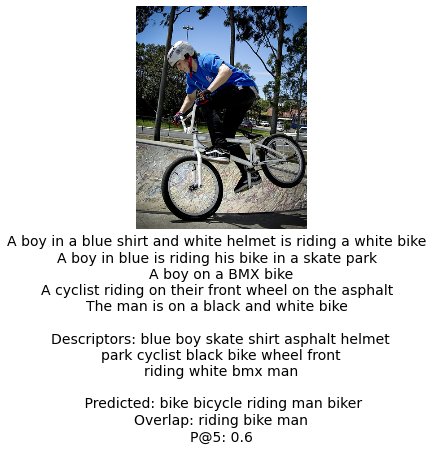
\includegraphics[scale=0.54]{chapters/TAL/bikeride}
\caption{\textit{Multiword image description example. Below the image
are the 5 captions describing the image, the union of words
that we take as targets, the top 5 predicted and the list of
correct words and the P@5 score for the given test case.}}
\label{fig:multiword-descriptors}
\end{figure}


\subsubsection{Single-concept image descriptions}
Even though we use separate portions of F8k and F30k for training and
testing, these subsets are still very similar. To test how general the
\textsc{Visual} word representations are, we use images from the ILSVRC2012
subset of ImageNet \citep{russakovsky2015imagenet} as benchmark. The major difference between these
images and the ones from F8k and F30k datasets is that labels of the
images in ImageNet are synsets from WordNet, which identify a single
concept present in the image instead of providing a natural
descriptions of its full content. Providing a quantitative evaluation
in this case is not straightforward for two main reasons. First, the
vocabulary of our model is restricted and the synsets in the ImageNet
dataset are quite varied. Second, the synset labels can be very precise,
much more so than the descriptions provided in the captions that we use
as our training data.

To attempt to solve the vocabulary mismatch problem, we use synset hypernyms
from WordNet as substitute target descriptors. If none of the lemmas
in the target synset are in the vocabulary of the model, the lemmas in
the hypernym synset are taken as new targets, until we reach the root
of the taxonomy. However, we find that in a large number of cases these hypernyms
are unrealistically general given the image. Figure \ref{fig:synset-descriptors}
illustrates these issues.

\begin{figure}
\centering
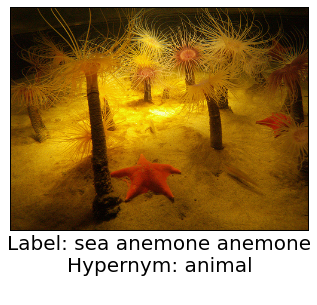
\includegraphics[scale=0.5]{chapters/TAL/starfish}
\caption{\textit{Example of the Single-concept image description task from
the validation portion of the ILSVRC2012 subset of ImageNet. The terms
"sea anemone" and "anemone" are unknown to \textsc{Visual} and "animal"
is the first word among it's hypernyms that appear in the vocabulary of F30k.}}
\label{fig:synset-descriptors}
\end{figure}

\section{Results}
\label{sec:results_intro}
We evaluate our model on two main tasks: simulating human judgments of
word similarity\footnote{We made available the source code used for running word similarity/relatedness
experiments on \url{https://bitbucket.org/kadar_akos/wordsims}.} and producing labels for images. For all performance measures in this sections (Spearman's $\rho$, P@5), we estimated the confidence intervals
using the Bias-corrected Accelerated bootstrapping method\footnote{
Provided by the scikits-bootstrap Python package \url{https://github.com/cgevans/scikits-bootstrap}.}
\citep{efron1982jackknife}.

\subsection{Word similarity}
\label{sec:res_wordsim}

We simulate the word similarity judgment task using the induced word
vectors by three models: \textsc{Visual}, \textsc{Monoling}, and
\textsc{Word2Vec}. All models were trained on the tokenized training
portion of the F30k data set. While \textsc{Visual} is presented
with pairs of captions and the 4,096 dimensional image-vectors,
\textsc{MonoLing} and \label{rev:word2vec}\textsc{Word2Vec}\footnote{We used the Word2Vec implementation from the
gensim Python package available at \url{https://radimrehurek.com/gensim/models/word2vec.html}.
} are trained solely on the sentences in the captions. The smoothing coefficient $\epsilon=1.0$ was used for
\textsc{Visual} and \textsc{Monoling}. The \textsc{Word2Vec} model was
run for one iteration with default parameters, except for the minimum
word count (as our models also consider each word in each sentence):
{\footnotesize feature-vector-size=100, alpha=0.025, window-size=5,
  min-count=5, downsampling=False, alpha=0.0001, model=skip-gram,
  hierarchical-sampling=True, negative-sampling=False}.


Figure~\ref{fig:wsj-online} illustrates the correlation of the similarity
judgments by the three models with those of humans on four
datasets. Table~\ref{table:wsj-online} shows the results in full detail:
it reports the Spearman rank-order correlation coefficient between the
human similarity judgments and the pairwise cosine similarities of the
word vectors per data set along with the confidence intervals
estimated by using bootstrap (the correlation values marked by a * were
significant at level $p<0.05$).\label{rev:wordsim_details}

Although \textsc{Visual} achieves a higher correlation than the other
two models on all datasets, \label{rev:variability} the overlapping confidence
intervals suggest that, in this particular setting, both
\textsc{Visual} and \textsc{Word2Vec} perform very similarly in
approximating human similarity judgments. This result is particularly
interesting as these models exploit different sources of information:
The input to \textsc{Word2Vec} is text only (i.e., the set of captions)
and it learns from word-word co-occurrences, while \textsc{Visual}
takes pairs of image vectors and sentences as input, and thus learns
from word-scene co-occurrences.

The significant medium-sized correlation ($p<.001$, $\rho=0.47$ 95\%
CI [0.44, 0.50]) with reasonably narrow confidence intervals on the
large number of samples, $N=2,839$, of the MEN data set supports the hypothesis
that the similarities between the meaning representations learned by \textsc{Visual}
mirror the distance between word pairs as estimated by humans.
This result suggests that it is feasible to learn word meanings from
co-occurrences of sentences with noisy visual scenes. However, on all other data sets,
the effect sizes for all models are small and their performances vary considerably given
different subsamples of the benchmarks.\label{ref:small_correlation}



\begin{figure}
\centering
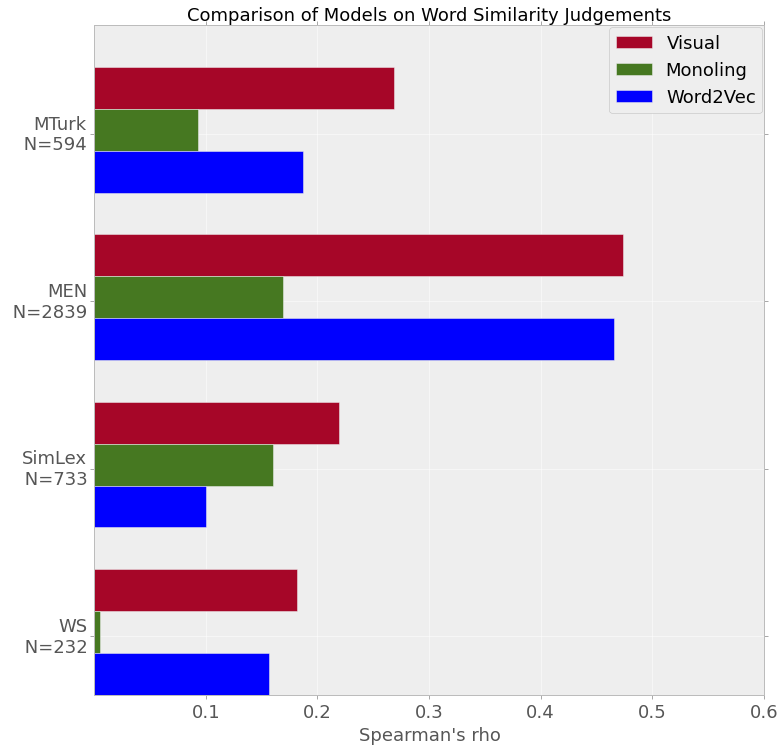
\includegraphics[scale=0.35]{chapters/TAL/modelcomparison}
\caption{\textit{Comparison of models on approximating word similarity
  judgments. The length of the bars indicate the size of the
  correlation measured by Spearman's $\rho$, longer bars indicate
  better similarity between the models' predictions and the human
  data. The labels on the y-axis contain the names of the data sets
  and indicate the number of overlapping word pairs with the
  vocabulary of the F30k data set. All models were trained on
  the training portion of the F30k data set.}}
\label{fig:wsj-online}
\end{figure}

\bgroup
\tabcolsep=0.11cm
%\def\arraystretch{1.5}
\begin{table}
{\small
\begin{tabular}{llllll}
\hline
{} &  WS &  SimLex &    MEN &  MTurk \\
\hline
\textsc{Visual}  &     {\bf 0.18*}  &   \bf{0.22}* &  \bf{0.47}* &
\bf{0.27}*\\
 {} & CI[0.05, 0.32] & CI[0.15, 0.29] & CI[0.44, 0.50] & CI[0.19, 0.34]\\
\textsc{Monoling}  &  0.08~ &   0.18* &  0.23* &  0.17*\\
 {} &  CI[-0.06, 0.21] & CI[0.11, 0.25] & CI[0.19, 0.26] & CI[0.04, 0.19]\\
\textsc{Word2Vec}           &  0.16* &   0.10* &  0.47* &  0.19* \\
{} &  CI[0.02, 0.28] & CI[0.02, 0.17] & CI[0.43  0.49]& CI[0.11, 0.26]\\
\hline
\end{tabular}
}
\caption{\textit{Word similarity correlations with human judgments measured by
  Spearman's $\rho$. Models were trained on the training portion of
  the F30k data set. The * next to the values marks the significance
  of the correlation at level $p<0.05$. The confidence intervals for
  the correlation are estimated using bootstrap.}}
\label{table:wsj-online}
\end{table}

\subsubsection{Concreteness}
\label{sec:concreteness}

Based on the previous findings of \cite{bruni2014multimodal}, we
expected that models relying on perceptual cues perform better on the
concrete portion of the word-pairs in the word-similarity
benchmarks. Furthermore, we expected approximating human word
similarity judgments on concrete word-pairs to be generally easier. As
discussed in section \ref{sec:effect-concrete}, we split the data sets
into {\it abstract} and {\it concrete} halves and ran the word
similarity experiments on the resulting portions of the word-pairs for
comparison. Table \ref{tab:conca} only reports the results on MEN and Simlex999 as these were
the only benchmarks that had at least 200 word-pairs after partitioning.
Table \ref{tab:benchmarks} summarizes the
average concreteness of the different portions of the data sets.


On all data sets, \textsc{Visual} seems to perform considerably better
on the concrete word-pairs then on abstract ones. On the abstract half of
the MEN data set, the performance of \textsc{Visual} is $\rho=0.35$,
95\% $CI[0.29, 0.41]$, while it is $\rho=0.56$, 95\% $CI[0.49, 0.59]$ on the
concrete portion. The non-overlapping confidence intervals support
the hypothesis that \textsc{Visual} does significantly better on the
concrete word pairs. This pattern, however, is not observed for
\textsc{Word2Vec} as there is no significant difference in its
performance given the different concreteness levels of the word pairs.
Splitting the word pairs in two groups based on their concreteness
scores reveals that performance of \textsc{Visual} is affected by
concreteness and that it only performs better than \textsc{Word2Vec}
on the more concrete word pairs.\label{rev:concrete-rank} Another
pattern that the analysis reveals is that the average concreteness of
the data sets is reflected in the performance of the models:
for both \textsc{Visual} and \textsc{Word2Vec} the rank of their performance follows the rank
of concreteness of the benchmarks.

\begin{table}
\centering
\small
\begin{tabular}{|c|c|c|c|c|c|}
\hline
       & \multicolumn{2}{|c|}{MEN} & \multicolumn{2}{c|}{SimLex} \\
\hline
	   &  Abstract & Concrete &  Abstract & Concrete \\
\hline
Visual & 0.35* & 0.55* &  0.16* & 0.39*  \\
& CI[0.29, 0.41] &CI[0.49, 0.59]  & CI[0.04, 0.25]& CI[0.28, 0.47] \\
\hline
Word2Vec & 0.48 & 0.45 &    0.14 & 0.18  \\
         &CI[0.43, 0.53]  &CI[0.39, 0.50] & CI[0.02, 0.25] & CI[0.07, 0.29]\\
\hline
\end{tabular}
\caption{\textit{The table reports the Spearman rank-order correlation coefficient
on the abstract and concrete portions of the data sets separately as
well as the confidence intervals around the effect-sizes estimated by using
bootstrap. The * next to the values indicates significance at level $p < 0.05$.}}
\label{tab:conca}
\end{table}

\begin{figure}
\label{fig:concreteness}
\centering
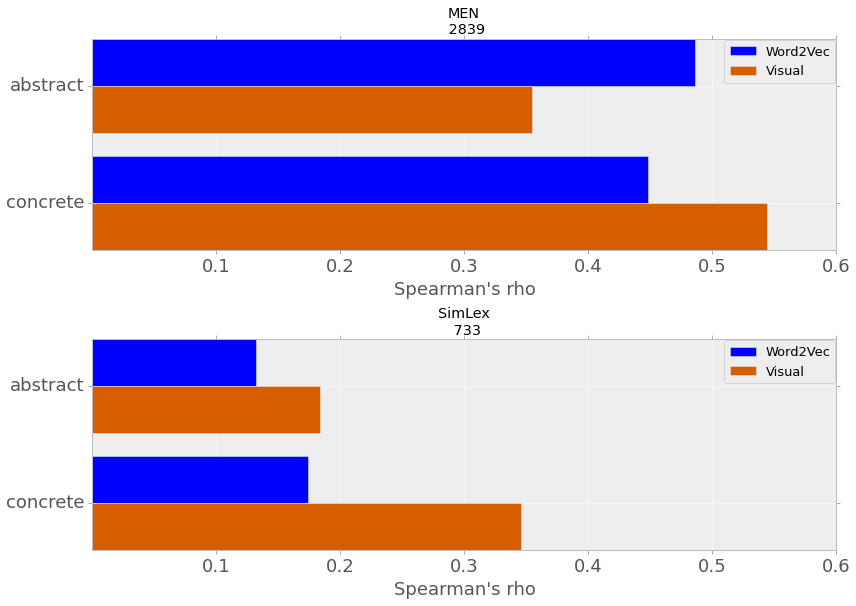
\includegraphics[scale=0.3]{chapters/TAL/concreteness}
\caption{\textit{Models' performance on word similarity
judgments as a function of the concreteness of the word pairs.}}
\end{figure}


\subsection{Word production}
In this set of experiments, we evaluate the word meaning vectors learned
by \textsc{Visual} by simulating the task of word production for an image, as described in
Section~\ref{sec:experiments-production}. These experiments can be viewed as
computational simulations of a language task where human subjects
associate words to given images. Words were ranked according to their
cosine similarity to a given image vector. The \textsc{Visual} model
was trained on the training portion of the F8k and F30k data
sets. We report results on two variations of the word production task:
multi-word image descriptors, and single-concept image descriptors.

\subsubsection{Multi-word image descriptors}
\label{sec:multi-word}
The objective of the model in this experiment is to rank only words in
the top $N$ that occur in the set containing all words from the
concatenation of the 5 captions of a given image with stop-words
removed. The ranking models used for these experiments (\textsc{Freq},
\textsc{Cosine}, and \textsc{Prior}) are described in
section \ref{sec:experiments-production}. Table \ref{tab:precision}
reports the results of the experiments on the respective test portions
of the F8k and F30k datasets as estimated by P@5.
We estimated the variability of the models'
performance by calculating these measures per sample and estimating
the confidence intervals around the means using bootstrap.

On these particular data sets the naive frequency
baseline can perform particularly well: by only retrieving the
sequence \emph{wearing, woman, people, shirt, blue} 
the ranking model \textsc{Freq} scores a P@5=.27
on F30k. Incorporating both the meaning representations learned by \textsc{Visual} and
the prior probabilities of the words, the non-overlapping
confidence intervals suggest that \textsc{Prior} significantly outperforms
\textsc{Freq} --- P@5=0.42, 95\% $CI [0.41, 0.44]$.

In addition to P@5, we also report the number of word types that
were retrieved correctly given the images (column Words@5 on table \ref{tab:precision}).
This measure was inspired by the observation that \label{rev:comined metric}
by focusing only on the precision scores it seems like
incorporating visual information rather than just using raw
word-frequency statistics provides a significant, but small
advantage. However, taking into consideration that \textsc{Prior}
retrieves 178 word types correctly suggests that it can retrieve less generic words that
are especially descriptive of fewer scenes.

\label{rev:intuitive multiword}To have a more intuitive grasp on the performance of \textsc{Prior}, it is
worth taking also into consideration the distribution of P@5 scores over the
test cases. When trained and tested on F30k in most cases (34\%), \textsc{Prior}
retrieves two words correctly in the top 5 and in 23\% and 25\% of the cases it retrieves one and
three respectively. In only 6\% of the time $P@5=0$,
which means that it is very unlikely that \textsc{Prior} named unrelated concepts
given an image.  These results suggest that \textsc{Visual} learns word meanings that
allow for labeling unseen images with reasonable accuracy using a large variety of words.

\begin{table}[h]
\centering
\begin{tabular}{|c|c|c|c|c|}
\hline
& \multicolumn{2}{|c|}{F8k} & \multicolumn{2}{|c|}{F30k} \\
\hline
 & P@5 & Words@5 & P@5 & Words@5 \\
\hline
\textsc{Freq}    & 0.20 & 5 &  0.27 &  5 \\
         &  CI[0.19, 0.21] & & CI[0.26, 0.29] & \\
\textsc{Cosine}  & 0.16 & 310 &  0.14 &  371\\
         &  CI[0.15, 0.17] & &  CI[0.13, 0.15] & \\
\textsc{Prior} & \bf{0.44}  & 135 &  \bf{0.42} & 178\\
         &  CI[0.42, 0.45] & &  CI[0.41, 0.44] &\\
\hline
\end{tabular}
\caption{\textit{Results for the multi-word image descriptors experiments
  reported on the test sets of F8k and F30k.  Words@5
  the number of correctly retrieved word types in
  the top 5. The confidence intervals below P@5 scores were
  estimated using bootstrap.}}
\label{tab:precision}
\end{table}


\subsubsection{Single-concept image descriptors}
The motivation for this experiment was to assess
the generalizability of the word-representations learned by \textsc{Visual}.
Similarly to the previous task, the goal here is to associate words to a
given image, but in this case the images are drawn from the
validation set of ILSVRC2012 portion of ImageNet
\citep{russakovsky2015imagenet}. Providing quantitative results is not as
straightforward as in the case of multi-word image descriptors, since
these images are not labeled with target descriptions, but with a
synset from WordNet. As demonstrated in Figure~\ref{fig:pretty}, some of
the lemmas in the target synsets are far too specific or unnatural for our
purposes, for example {\it schooner} for an image
depicting a sailboat or {\it alp} for an image of a mountain.
In other cases, a particular object is named which
might not be the most salient one, for example {\it freight car} for a
picture of a graffiti with three pine trees on the side of railway carriage.

We made an attempt to search through the lemmas in the hypernym paths
of the synsets until a known target lemma is reached. However, as
demonstrated by examples in Figure\~ref{fig:pretty}, these hypernyms are
often very general (e.g.\ {\it device}) and predicting such high-level
concepts as descriptors of the image is unrealistic. In other cases,
the lemmas from the hypernym synsets are simply misleading; for
example, {\it wood} for describing a wooden wind instrument. As can be
seen in the examples in Figure~\ref{fig:pretty}, the top ranked words
predicted by our model are in fact conceptually more similar to the
images covering a variety of objects and concepts than the labels
specified in the dataset.

%\ignore{
%\begin{figure}
%\centering
%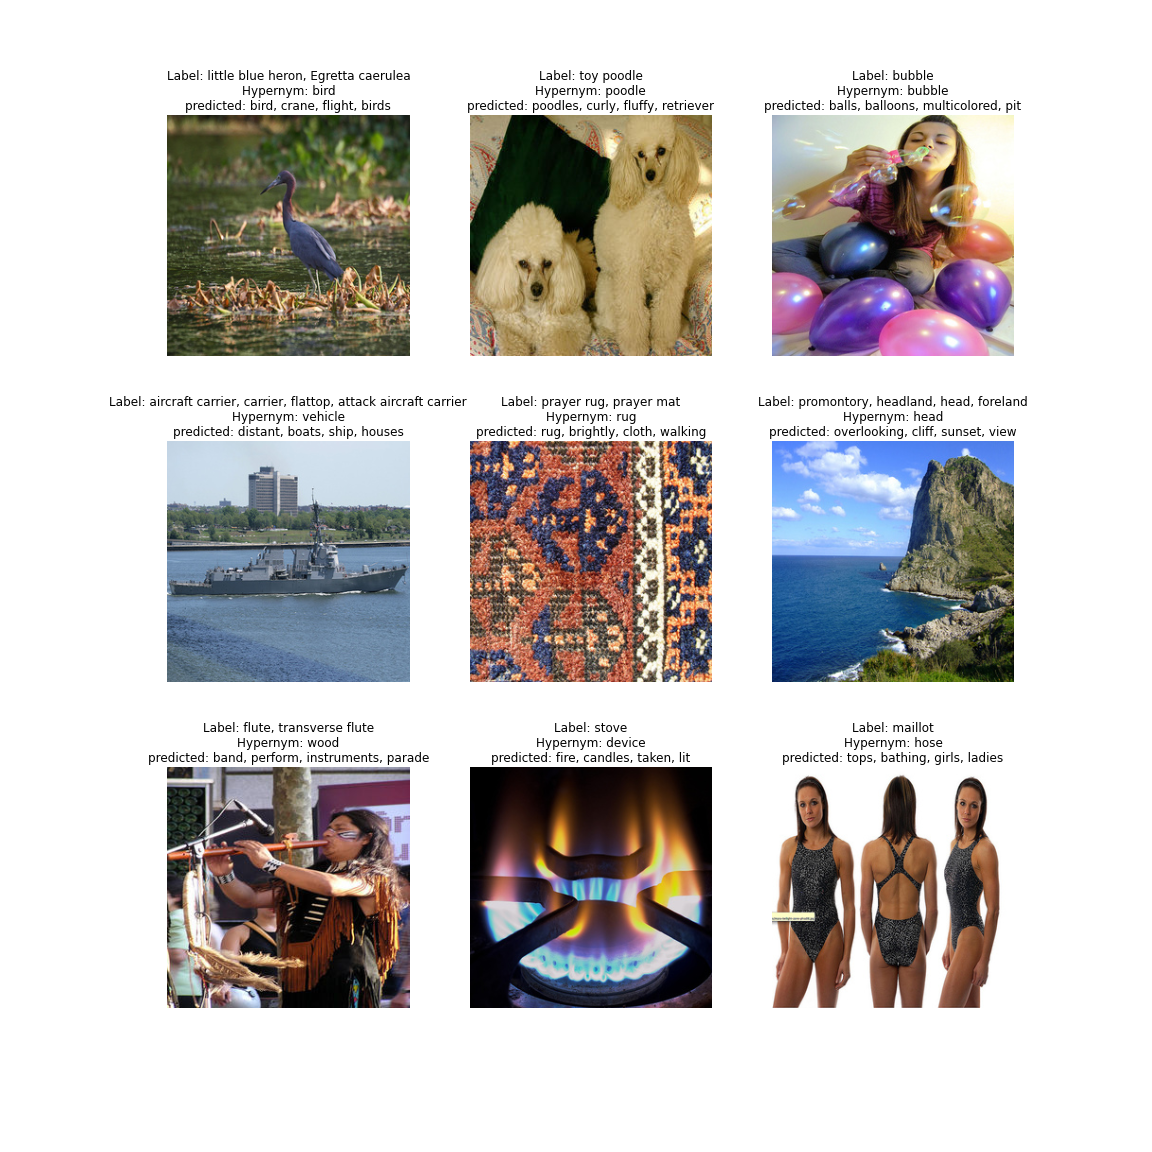
\includegraphics[scale=0.3]{chapters/TAL/pretty_pictures}
%\caption{\textit{The caption above the images show the target labels, the
%  hypernyms that were considered as a new target if the original was
%  not in the vocabulary and the top $N$ predicted words. In a large
%  number of cases the guesses of the model are conceptually similar to
%  the images, although, do not actually overlap with the labels or the
%  hypernyms.}}
%\label{fig:pretty}
%\end{figure}
%}


\begin{figure}
\centering
\tabcolsep=0.08cm
\begin{tabular}{ccc}
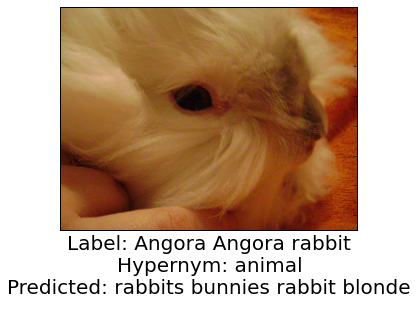
\includegraphics[scale=0.23]{chapters/TAL/imagenet/bunny} & 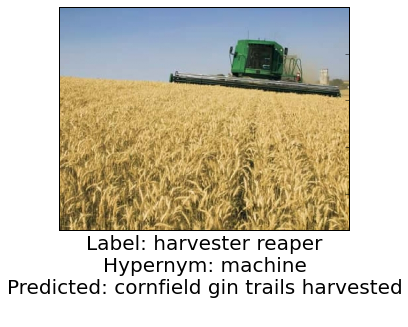
\includegraphics[scale=0.23]{chapters/TAL/imagenet/corn} & 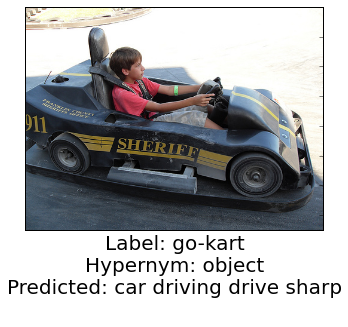
\includegraphics[scale=0.23]{chapters/TAL/imagenet/gocart} \\
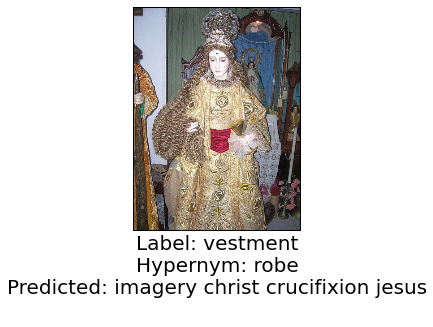
\includegraphics[scale=0.23]{chapters/TAL/imagenet/mary} & 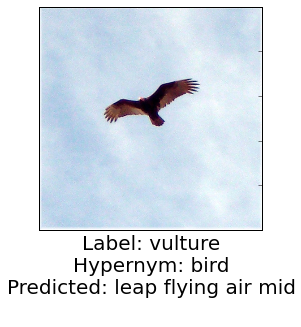
\includegraphics[scale=0.23]{chapters/TAL/imagenet/eagle} & 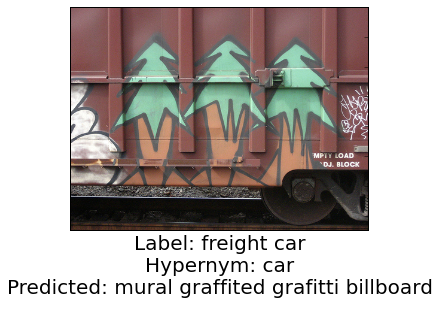
\includegraphics[scale=0.23]{chapters/TAL/imagenet/graffiti} \\
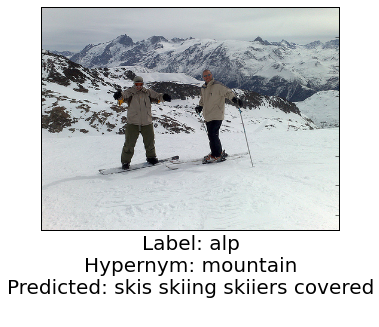
\includegraphics[scale=0.23]{chapters/TAL/imagenet/ski} & 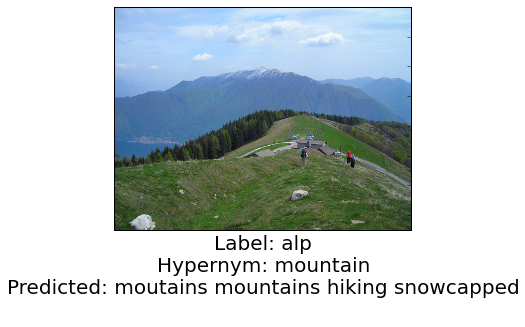
\includegraphics[scale=0.23]{chapters/TAL/imagenet/mountain} & 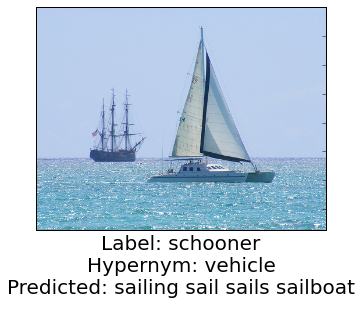
\includegraphics[scale=0.23]{chapters/TAL/imagenet/sail}
\end{tabular}
\caption{\textit{The caption above the images show the target labels, the
  hypernyms that were considered as a new target if the original was
  not in the vocabulary and the top $N$ predicted words. In a large
  number of cases the guesses of the model are conceptually similar to
  the images, although, do not actually overlap with the labels or the
  hypernyms.}}
\label{fig:pretty}
\end{figure}

We conclude that in the future, to quantitatively investigate the cognitive plausibility of cross-situational
models of word learning, the collection of feature production norms for ImageNet \citep{russakovsky2015imagenet} would
be largely beneficial.

\section{Discussion and conclusion}
\label{sec:discussion}

We have presented a computational cross-situational word
learning model that learns word meanings from pairs
images and their natural language descriptions. Unlike
previous word learning studies which often rely on artificially
generated perceptual input, the visual features we extract from images
of natural scenes offers a more realistic simulation of the cognitive
tasks humans face, since our data includes a significant level of
ambiguity and referential uncertainty.

Our results suggest that the proposed model can learn meaningful
representations for individual words from varied scenes and their
multiword descriptions. Learning takes place incrementally and without
assuming access to single-word unambiguous utterances or corrective
feedback.  When using the learned visual vector representations for
simulating human ratings of word-pair similarity, our model shows
significant correlation with human similarity judgments on a number of
benchmarks. Moreover, it moderately outperforms other models that only
rely on word-word co-occurrence statistics to learn word meaning.

The comparable performance of visual versus word-based models seems to
be in line with \cite{louwerse2011symbol}, who argues that linguistic
and perceptual information show a strong correlation, and therefore
meaning representations solely based on linguistic data are not
distinguishable from representations learned from perceptual
information. However, an analysis of the impact of word concreteness
on the performance of our model shows that visual features are
especially useful when estimating the similarity of more concrete word
pairs. In contrast, models that rely on word-based cues do not show such improvement
when judging the similarity of concrete word pairs. These results
suggest that these two sources of information might best be viewed as
complementary, as also argued by \cite{bruni2014multimodal}.

We also used the word meaning representations that our model learns
from visual input to predict the best label for a given image. This
task is similar to word production in language learners. Our
quantitative and qualitative analyses show that the learned
representations are informative and the model can produce intuitive
labels for the images in our dataset. However, as discussed in the
previous section, the available image collections and their labels
are not developed to suit our purpose, as most of the ImageNet
labels are too detailed and at a taxonomic level which is not
compatible with how language learners name a visual concept.

% In the future, we plan to collect a dataset of pictures labeled by
% humans ???\todo{I don't know what to promise here!}.

Finally, a natural next step for this model is to also take into
account cues from sentence structure. For example,
\cite{alishahi2012concurrent} try to include basic syntactic
structure by introducing a separate category learning module into
their model.  Alternatively, learning sequential structure and visual
features could be modeled in an integrated rather than modular
fashion, as done by the multimodal captioning systems based on
recurrent neural nets (see section~\ref{subsec:meanings-from-images}).
We are currently developing this style of integrated model
to investigate the impact of structure on word learning from a
cognitive point of view.


%\bibliographystyle{apalike}
%\bibliography{refs}

%\newpage
\pagenumbering{roman}

\noindent
Dear Dr.~Merlo,
\newline

Thank you for the very helpful suggestions and insightful questions
posed in this review.  We apologize for the delay getting this
revision back to you and very much appreciate the extension you 
gave us to resubmit the manuscript.

We have substantially revised the article in response to your and the reviewers' 
comments. Specifically with regard to the two main issues you raised, we have 
introduced a uni-modal language model (referred to as the {\sc LM} model in the text) 
and reported the results of the experiments on this model as well. Also following 
your recommendation, we have removed the exploratory parts of (the old) Section 6, 
and reorganized the paper by merging previous Sections 4, 5 and the remaining of 
Section 6 into a single section containing all the experiments (that is Section 4 in the 
revised manuscript). We have kept and expanded the quantitative analysis of the nature of 
n-gram contexts that trigger individual dimensions in the hidden layers; this experiment is 
now reported in Section~\ref{sec:contexts}.

Furthermore, we have made clarifications about the details of the techniques all 
through the manuscript, expanded Introduction (Section~\ref{sec:intro}) to 
emphasise our contributions, updated Related Work (Section~\ref{sec:related}) 
to include relevant papers that came out while this manuscript was under review, and 
expanded Discussion (Section~\ref{sec:conclusion}) to discuss in more detail the 
relevance and generalizability of our techniques. 
We reran all the experiments with a different, more reliable parser,
which caused minor differences in the details of the figures.

We believe that the revisions to the paper address your collective
concerns, and we thank you all again for the comments that have helped
us to improve the paper.
\newline

\noindent
Sincerely,
\newline

\noindent
Ákos Kádár, Grzegorz Chrupała and Afra Alishahi
\newline


\begin{verbatim}
Dear Ákos Kádár:

We have reached a decision regarding your submission to Computational
Linguistics, "Representation of linguistic form and function in
recurrent neural networks". I include here the reviews for your
perusal.

The reviewers and I like the area of work in which this paper is
situated: model analysis. While the reviews correctly point out that
several shortcomings remain, a discussion has identified the
modifications that we think are really required, to make the paper
stronger. Other ideas are suggestions that we leave to you for future
work.

The requested changes concern an added comparisons to unimodal models
(or at least to unimodal versions of Imaginet). On the other hand, all
the reviewers thought that Section 6 is less convincing than the rest
of the paper, at least in the current writeup. So we think that this
Section could be reduced in favor of adding the unimodal experiments .

I would be grateful if you could provide an appropriately revised
version of your paper by 10th February 2017. Please email the
editorial assistant (editorialoffice@cljournal.org) within one week,
to confirm whether you will be able to meet this target date, or to
negotiate a new target date.

You will find details of the resubmission process at
http://cljournal.org/ojs-help.html.  When you submit your revised
paper, please enclose a letter that responds specifically to each of
the points made by the reviewers, outlining the changes you have made,
and those you have not addressed, together with an electronic copy of
the revised manuscript as a PDF file.

Thank you for submitting to Computational Linguistics.


Paola Merlo
University of Geneva
Paola.Merlo@unige.ch
------------------------------------------------------
Reviewer A:


2 What is this paper about? [Help] :
The paper presents methodologies for analyzing what is learned by
recurrent neural networks. It does this by suggesting two
methodologies, and then applying them to two similar tasks -- one that
that is based on language modeling, and another which is based on
visual recognition. The analysis highlights some of the things that
are encoded and not encoded in each of the representations.


3 Strengths and Weaknesses [Help]

Strengths:

The topic of understanding what is learned by neural network models,
in particular recurrent ones, is of great importance and interest, and
papers of this kind are very much needed. While most work tries to use
"deep learning" and RNNs to "improve" on various language tasks,
understanding their capabilities and inner working, and making them
more transparent, is much more challenging, and there are not enough
works in this area. The current work attempts to do precisely that,
and it also delivers on its promise with an interesting methodology
and insights. In particular, the first part (section 5) is
particularly well done. Section 6 is somewhat less convincing, but
still is on-par or better than any other work that attempts to deliver
analysis and insights.


Weaknesses:
 
Some parts of the papers were not clear, and could be improved. I also
have someissues with some of the experiments in section 6, which can
either be presented better or even removed altogether, in my view.

- In terms of clarity, I would appreciate a better description of the
  IMAGINET model, which is being analyzed. The model is described in
  terms of its equations, but I would like to see a better
  presentation of what is the intent behind it -

- what is being modeled and what is being learned? this is available
  in the original IMAGINET paper, but I think the description should
  be imported to this paper also, in order to make it self contained
  and stronger.
  
\end{verbatim}  
\begin{quote}
\textsc{Author Response:}
We have expanded Section~\ref{sec:imaginet} with a conceptual
description of {\sc Imaginet} and its learning goals, and added a graphical
representation of the structure of the model for more clarity (Figure~\ref{fig:imaginet}).
\end{quote}
\begin{verbatim}

- Also in terms of clarity, the graphs are not described in enough
  detail in my view. Whiel the box plots (figure 2 and others) are
  somewhat standard, they are not mainstream in the NLP commuity, and
  I would appreciate seeing a more detailed description in the main
  text or the caption of what each component means, both generally and
  in the context of the specific graph.
\end{verbatim}  
\begin{quote}
\textsc{Author Response:}  We have provided an interpretation of the boxplots 
in footnote~\ref{ft:boxplots} on page~\pageref{ft:boxplots}.
\end{quote}
\begin{verbatim}
- Figure 7 is confusing -- what are the different colors between,
  e.g., the words "in" and "tree" in the first line, and between "a"
  and "wii" in the second? I assume this is some "gradient" between
  two colors, but it looks like there are several data points and is
  very confusing. Please fix this.
\end{verbatim}  
\begin{quote}
\textsc{Author Response:}  Following the recommendation of the reviewers,
we shortened the original Section 6 and removed this figure.
\end{quote}
\begin{verbatim}

In terms of content:

- In section 6.1, why is the sorting by magnitude and not by absolute
  value? are negative activations not important?
\end{verbatim}  
\begin{quote}
\textsc{Author Response:}  It was in fact the absolute value of the activations 
that was taken into account. In the revised manuscript, we have removed this 
and other exploratory experiments and expanded the quantitative analyses.
\end{quote}
\begin{verbatim}

- When choosing the "top k context of each unit" (section 6.1), it is
  not clear what a "unit" is and how it is chosen.
\end{verbatim}  
\begin{quote}
\textsc{Author Response:}  A unit is one individual dimension in the final hidden layer 
of the network. We have made this clear in the revised text.
\end{quote}
\begin{verbatim}

- I did not understand the last sentence in section 6.1, and would
  appreciate an elaboration on this point (or a removal).
\end{verbatim}  
\begin{quote}
\textsc{Author Response:}  We removed this part and added an 
expanded discussion of the generalizability of our techniques to 
Discussion (Section~\ref{sec:conclusion}).
\end{quote}
\begin{verbatim}

- In section 6.2, it is not clear how trigrams with high activations
  are chosen. How is a trigram with high activation defined? this is
  not clear from the description of the method.
\end{verbatim}  
\begin{quote}
\textsc{Author Response:} We have removed this section in the revised manuscript. We 
address the nature of contexts which trigger individual dimensions and a systematic
procedure for selecting the dimensions themselves in more detail now in 
Section~\ref{sec:contexts}.
\end{quote}
\begin{verbatim}

- I am not convinced by the experiments in section 6.3 and their
  importance -- either they are not described properly and I missed
  something, or they are somewhat meaningless: when training a
  logistic regression model to predict grammatical function, it is not
  surprising that ones finds units that are predictive of grammatical
  function.
\end{verbatim}  
\begin{quote}
\textsc{Author Response:}  As mentioned before, we have reorganised 
the experiments and removed the exploratory parts, including the old Section 6.3. 
We address the issue of encoding grammatical functions in the revised manuscript in 
Sections ~\ref{sec:beyondlexical} (specifically in \ref{sec:gramfunc}).
\end{quote}
\begin{verbatim}


~ Where is section 6.4?

\end{verbatim}  
\begin{quote}
\textsc{Author Response:} It was there, believe us! But we have removed this 
experiment from the revised version for the sake of clarity and coherence of our analyses.
\end{quote}
\begin{verbatim}

~ a related (unpublished, but available on arxiv) work is
https://arxiv.org/abs/1608.04207

\end{verbatim}  
\begin{quote}
\textsc{Author Response:}  We have expanded the discussion of related work 
(Section~\ref{sec:related}) and included this work in addition to a few others which 
came out while our submission was under review.
\end{quote}
\begin{verbatim}

4 Substantive Revisions Required [Help]

Complete this section if either 'Revise and Resubmit' or 'Reject' has
been recommended.

Revisions to be Required:
: 



Revisions to be Encouraged:
: 



5 Minor Revisions Required [Help]
:

See the points marked with (-) in the weaknesses above. Points marked
with (~) are less important. For section 6.3, my recommendation is
that it is either substantially revised, or removed altogether -- I
believe the paper has enough merit without it.

\end{verbatim}  
\begin{quote}
\textsc{Author Response:}  We hope we have addressed all your comments and concerns. We have removed the experiments in (the old) Section 6.3 from the revised manuscript.
\end{quote}
\begin{verbatim}

6 Typographic Errors [Help]
:

- "by as" in the first sentence of the intro.

- There are some cases of using parenthesis in citation where they
  shouldn't be, for example the first two citations in section 2 ("of
  (Elman 1990)" should be "of Elman (1990)").

\end{verbatim}  
\begin{quote}
\textsc{Author Response:} The typo and the citation inconsistencies are fixed.
\end{quote}
\begin{verbatim}

------------------------------------------------------

------------------------------------------------------
Reviewer E:


2 What is this paper about? [Help]
: 

The paper presents a set of methods for analyzing the activations of
recurrent neural networks from a linguistic perspective using:

a) omission scores (to examine the contribution of a single token to
the prediction of the network); and

b) top k contexts (keeping the activations for the entire sequence and
examining individual dimensions)

The model used in this paper is a multimodal (text and visual)
multi-task RNN (Imaginet). At each time step the next word is
predicted from its current state, and an image vector is predicted
from the model's final state. The model consists of two parallel GRUs
with shared word embeddings.

By pairing omission scores with POS and dependency relations, the
authors show that the Visual pathway mostly focuses on noun and noun
relations, while the textual pathway focuses more on function
words. The textual pathway has in general a more uniform omission
score distribution, the visual model peaks on content words (albeit
not particularly on verbs, as the authors discuss).


3 Strengths and Weaknesses [Help]

Strengths:
: 
* neat idea and novel contribution (pairing activations with POS and
dependency relations to gain further insights into RNNs)

* extensive analysis; especially going beyond lexical cues (Section
5.3), where the authors train a regression model to predict omission
scores on a token level, showing that the network not just learns to
rely on word types, but it also learns position information
(particularly important for the textual pathway)


Weaknesses:
: 
* the description of the top K contexts is not clear, how are top k
contexts calculated? do you find the most active token (highest
absolute value of hidden activation in the sequence?) and then use
the words around it to find the trigrams? (what is meant by 'each
unit' in Section6.1? Is the matrix actually R^nxd?); maybe you sort
by column, not row? 

\end{verbatim}  
\begin{quote}
\textsc{Author Response:}  You are absolutely right about the description of 
top k contexts being confusing. We have removed this part and reorganized 
the experiments section (Section~\ref{sec:experiments}) to make it more understandable
and coherent. 
\end{quote}
\begin{verbatim}

* Section 6.5 shows that the visual pathway focuses more on dependency
relations, supporting the finding in the omission score part;
however, the section is again very dense and Figure 7 only shows
activations for Visual; I'd suggest to drop this part from the paper

\end{verbatim}  
\begin{quote}
\textsc{Author Response:}  Following your and others' suggestion, we have removed this section from the revised manuscript.
\end{quote}
\begin{verbatim}

4 Substantive Revisions Required [Help]

Complete this section if either 'Revise and Resubmit' or 'Reject' has
been recommended.

Revisions to be Required:
: 
- clearer description of how top k contexts are obtained
\end{verbatim}  
\begin{quote}
\textsc{Author Response:}  As mentioned above, we have removed this part and reorganized Section~\ref{sec:experiments} to make our analyses more concrete and clear.
\end{quote}
\begin{verbatim}


Revisions to be Encouraged:
: 
- figures are not readable in BW printing; in addition to color, use
  different symbols/line types
\end{verbatim}  
\begin{quote}
\textsc{Author Response:}  We have reformatted many of our figures to make them more readable.
\end{quote}
\begin{verbatim}

- Related Work: clarify better how you differ from Li et al. (2015),
  you mention "for a comparative analysis": I interpret this as "we
  analyze a multi-task learning model (visual / textual) and compare
  what the two parts learn"
\end{verbatim}  
\begin{quote}
\textsc{Author Response:} We have edited our related work section to make the comparison more 
clear. In addition to taking into account tasks that rely on different modalities (language as well as vision), 
we focus more on learning structural properties of the input, whereas Li et al. (2015) focus on single
tokens.
\end{quote}
\begin{verbatim}


5 Minor Revisions Required [Help]
: 
- Sec 2, clarify: what are 'negative strings'? (non-words?)
\end{verbatim}  
\begin{quote}
\textsc{Author Response:}  we have reworded `positive' and `negative' as `grammatical' 
and `ungrammatical' to avoid confusion.
\end{quote}
\begin{verbatim}
- Before equation 9 missing lambda ("weighted by \lambda"; what lambda
  is used in the exp.?)
\end{verbatim}  
\begin{quote}
\textsc{Author Response:}  There was no lambda in that equation, but in 
Section~\ref{sec:imaginet} we report the value we use for the parameter 
$\alpha$ in Equation~(\ref{eq:losscombo}).
\end{quote}
\begin{verbatim}
- it would be helpful to include a figure of model (as in original
  paper)
\end{verbatim}  
\begin{quote}
\textsc{Author Response:}  We have included an illustration of the structure of the 
model in Figure~\ref{fig:imaginet}.
\end{quote}
\begin{verbatim}
- "two minor modifications" but the first seems you also use cosine,
  was that different previously, not clear.
\end{verbatim}  
\begin{quote}
\textsc{Author Response:}  You are right, the description of the model in 
Section~\ref{sec:imaginet} presents the version used in this paper, which uses 
cosine distance. The original Imaginet model uses mean square error instead; 
we clarified this issue in footnote~\ref{ft:imaginet}.  
\end{quote}
\begin{verbatim}
- specify interaction features in regression model
\end{verbatim}  
\begin{quote}
\textsc{Author Response:}  We have specified the interaction features used in each regression model in Section~\ref{sec:beyondlexical}.
\end{quote}
\begin{verbatim}
- 5.3.1. why also 'water'?
\end{verbatim}  
\begin{quote}
\textsc{Author Response:}  We have removed {\it water} from the set of examples 
in Figure~\ref{fig:top_words}.
\end{quote}
\begin{verbatim}


6 Typographic Errors [Help]
: 
- abstract: sentence "Based on.." way too long
- mention multi-task in abstract
- introduction: "this includes various" > "This can be applied to
  various"
- from linguistic point (missing det)
- generally avoid long sentences (e.g., last paragraph sec 5.1,
  sec. 5.2)
- rephrase: "this model we refer to as SUM"
- windowsizes
\end{verbatim}  
\begin{quote}
\textsc{Author Response:}  We have fixed these issues, thanks for bringing them to our attention.
\end{quote}
\begin{verbatim}

------------------------------------------------------

------------------------------------------------------
Reviewer F:


2 What is this paper about? [Help]
: 
This paper presents an analysis of the information learned by
recurrent neural networks. It focuses on one particular multimodal,
multitask model, Imaginet, which is trained on images and their
descriptions. The paper proposes a new measure, the omission score,
which indicates how sensitive the network is to individual words in
the input. Using this method, the authors show that the textual module
of the model pays attention to function words, while the visual module
pays attention to content words. The authors then propose a second
method which can be used to analyze which n-grams the hidden units of
the model are sensitive to; this results in meaningful syntactic and
semantic clusters. This time, there is no clear-cut distinction
between textual and visual modules.


3 Strengths and Weaknesses [Help]

Strengths:
: 
This paper makes a useful methodological contribution by proposing
methods to analyze the knowledge learned by neural networks, which is
an underexplored area, at least for networks trained on text data. The
paper is well written, and technically sound.


Weaknesses:
: 
The results of the paper are unfortunately fairly obvious. From the
omission score analysis, we learn that a model trained to predict the
next word in a sentence is sensitive to function words, while a word
trained to associate a sentence with an image representation (which is
essentially the output of the object detector) pays more attention to
nouns. This is not at all surprising, it just reflects the different
training objectives. The fact that the hidden units respond to
specific n-grams is also expected; most people already believe that
RNNs are good at approximating n-gram models; the question is, can
they model more elaborate syntactic structures?
\end{verbatim}  
\begin{quote}
\textsc{Author Response:}  
The results from Figure~\ref{fig:omission-imaginet} are indeed
unsurprising. We should expect any method which works well to recover
such expected results. In addition, however, there are other findings
which we consider far from obvious: for example the fact that the
{\sc Visual} pathway assigns very different importance to the same
word type in different grammatical functions (see See
Section~\ref{sec:beyondlexical}). We have tried to highlight the
non-trivial insights more in the paper. 


%\todo[inline]{address}
\end{quote}
\begin{verbatim}

This is really the question that the authors should explore, e.g., by
testing whether the model can learn long distance dependencies,
agreement, recursion, word order. An example for recent work that goes
in this direction is Linzen et al. (2016).
\end{verbatim}  
\begin{quote}
\textsc{Author Response:} We have expanded the related work 
(Section~\ref{sec:related}) with a discussion of Linzen et al. (2016) 
and a few other relevant articles that came out while our submission was under review.
\end{quote}
\begin{verbatim}

Another limitation of the paper is its focus on one particular model,
which happens to be the authors'. To be convincing, the paper would
really need to compare results for this model with results for other
architectures, showing that the proposed analysis methods offer real
discriminative power.
\end{verbatim}  
\begin{quote}
\textsc{Author Response:}  Due to space and time limitations we have to 
leave the comparison with other architectures for future work; however we 
have expanded the discussion of the generalizability of our techniques to other
architectures in Discussion (Section~\ref{sec:conclusion}).
\end{quote}
\begin{verbatim}

Related to this, it is not clear to me why a multimodal, multitask
model such as Imaginet is required for the work presented
here. Surely, similar results would be obtained if two unimodal RNN
models were trained, one on image descriptions to predict the next
word, and one on image representations to predict the description.
\end{verbatim}  
\begin{quote}
\textsc{Author Response:}  The motivation for using {\sc Imaginet} is laid
out in the introduction. The main point is that this model consists of
two loosely coupled pathways: One ({\sc Textual}) is a language
model which is a type of network widely used and reasonably well
understood. The other one ({\sc Visual}) is a visually-grounded encoder,
a much less commonly used and studied type of network. By using {\sc
  Imaginet} we can apply our methods to these two network types and
compare the results head-to-head. Thus {\sc Textual} serves
mostly to show that our methods give reasonable, expected answers,
while with {\sc Visual} we can generate novel, previously unfamiliar
insights. The multitask setup is not strictly
necessary for this; in order to abstract away from the effect of multitask
training on {\sc Textual} we have now added experiments on a
standalone language model {\sc LM}.

%\todo[inline]{address}
\end{quote}
\begin{verbatim}

4 Substantive Revisions Required [Help]

Complete this section if either 'Revise and Resubmit' or 'Reject' has
been recommended.

Revisions to be Required:
: 
(1) Add comparisons to unimodal models (or at least to unimodal
versions of Imaginet).
\end{verbatim}  
\begin{quote}
\textsc{Author Response:}  In the revised manuscript we have introduced a uni-modal language model, and updated all of our experiments to include this model as well.
\end{quote}
\begin{verbatim}

(2) Add comparisons to other architectures (LSTMs, etc.)
\end{verbatim}  
\begin{quote}
\textsc{Author Response:}  As we mentioned before, we are very interested in 
applying our proposed techniques to other tasks and architectures in future work. 
For the sake of this manuscript, we have included a theoretical discussion of how 
these techniques can be implemented for a number of other architectures (see 
Section~\ref{sec:conclusion}).
\end{quote}
\begin{verbatim}

(3) Sec. 5.3.2 should be cut. You don't have connected discourse, just
isolated sentences. So it is purely speculative to say these
observations are due to topic/content structure, rather than just to
linear order.
\end{verbatim}  
\begin{quote}
\textsc{Author Response:}  Our explanation of the aim of this experiment in the original version might have been misleading; we have rewritten this section to make it clear that we are examining the information structure within a single sentence and not in a dialogue. We do believe that the results we report in this section are interesting and nontrivial, especially the fact that the position usually occupied by the subject of the sentence is the most important for the {\sc Visual} model despite the common recency bias in RNNs.
\end{quote}
\begin{verbatim}

(4) The paper relies too much on impressionistic evaluation based on
suggestive figures, rather than on quantitative analysis. An exception
is Fig. 8. There should be more of this type of analysis.
\end{verbatim}  
\begin{quote}
\textsc{Author Response:}  We have removed the exploratory parts of (the old) Section 6, and expanded the quantitative analysis of the nature of triggering contexts in Section~\ref{sec:contexts}. 
\end{quote}
\begin{verbatim}

(5) The authors should discuss the recent paper by Linzen et
al. (2016). This is a good example for an attempt to evaluate
linguistic structure learned by an RNN that goes beyond individual
words or n-grams.
\end{verbatim}  
\begin{quote}
\textsc{Author Response:}  As mentioned before, we have included a discussion of
this paper in our related work.
\end{quote}
\begin{verbatim}

Reference

Assessing the Ability of LSTMs to Learn Syntax-Sensitive
Dependencies. Tal Linzen, Emmanuel Dupoux, Yoav Goldberg. To appear in
TACL 2016. https://arxiv.org/abs/1611.01368v1


Revisions to be Encouraged:
: 



5 Minor Revisions Required [Help]
: 



6 Typographic Errors [Help]
: 

------------------------------------------------------
\end{verbatim}



%\end{document}

%%% Local Variables:
%%% mode: latex
%%% TeX-master: t
%%% End:
